\documentclass[tikz]{standalone}
\usetikzlibrary{calc}
  \usepackage[no-math]{fontspec}
  \setmainfont{TeXGyreTermes-Regular}[
       BoldFont       = TeXGyreTermes-Bold ,
       ItalicFont     = TeXGyreTermes-Italic ,
       BoldItalicFont = TeXGyreTermes-BoldItalic,
       NFSSFamily     = ntxtlf]
  \setsansfont{TeX Gyre Heros Regular}[
       Scale=.9,
       BoldFont       = TeX Gyre Heros Bold,
       ItalicFont     = TeX Gyre Heros Italic,
       BoldItalicFont = TeX Gyre Heros BoldItalic]
  \setmonofont[StylisticSet={1,3},Scale=.9]{inconsolata}
  \usepackage{newtxmath}
\begin{document}

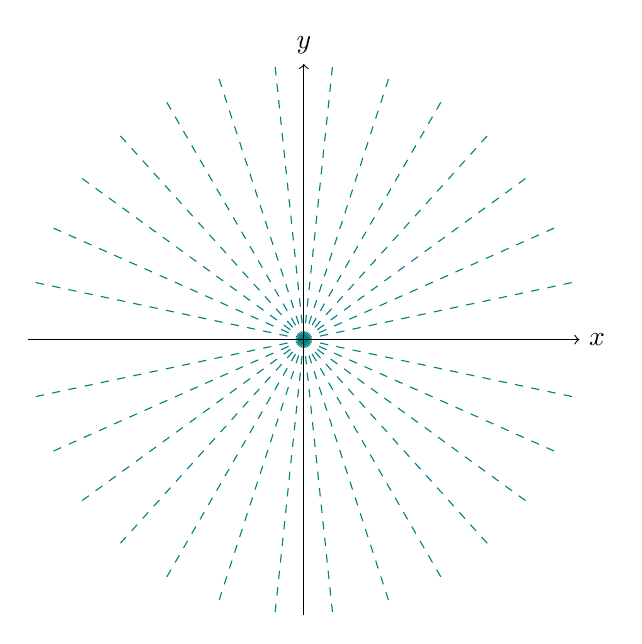
\begin{tikzpicture}
\def\xmax{3} \def\xmin{-3}
\def\ymax{3} \def\ymin{-3}
\def\r{3.5}

\def\n{30}
\def\h{360 / \n}

\foreach \a in {0,...,\n}
        \draw[teal, dashed, thin] 
        (0,0) -- ({\r * cos(\h * \a)}, {\r * sin(\h * \a)}); 

\draw[->] (\xmin-.5,0)--(\xmax+.5,0) node[right] {$x$};
\draw[->] (0,\ymin-.5)--(0,\ymax+.5) node[above] {$y$};
\end{tikzpicture}
\end{document}